\chapter{Techniques de fabrication de structures en salle blanche}
\label{Chap2}
    Pour réaliser la structure que l'on souhaite à partir des nanofils, il va falloir utiliser différentes méthodes de salle blanche. De plus, avant même de commencer à travailler sur de vrais échantillons, il est important de réaliser des tests avec des structures de test, pour savoir si le processus que l'on veut mettre en place est viable.
    
    \section{Résines}
    Point central de la fabrication, les résines permettent de créer le dessin que l'on souhaite obtenir sur le wafer.
        \subsection{De la théorie...}
            Les résines que nous allons utiliser sont composées de matériaux polymères : le Polymethyl Methacrilate (PMMA) (Fig. \ref{PMMA}) et copolymères Methyl Methacrilate (MMA). 
            
            \begin{figure}
            \centering
            \chemfig{CH_3-[:270]C(=[:180]CH_2)(-[:270]C(=[:0]O)(-[:270]O(-[:315]CH_3)))}
            \caption{Structure chimique du MMA, le monomère qui compose le PMMA}
            \label{PMMA}
            \end{figure}
            
            Il existe bien sur d'autres types de résines, notamment sensibles à la lumière (photorésines) davantage utilisées pour les processus de fabrication impliquant des semiconducteurs.
            
            Les résines que nous utilisons sont sensibles aux électrons : Envoyer un faisceau d'électrons de haute énergie (Voir \ref{explicationebl}) impliquera des modification structurelles. Pour le PMMA par exemple, le faisceau d'électrons brise le polymère en monomères beaucoup plus solubles dans le Methyl IsoButyl Ketone (MIBK) (Fig. \ref{MIBK}). Les résines sont liquides et déposées au centre du wafer. On place ensuite celui-ci dans un spinner, qui va tourner et répartir la résine de manière uniforme sur le wafer. 
            
            \begin{figure}
                \centering
                \chemfig{-[:-30](-[:30]-[:-30](-[:30])(=[:270]O))(-[:270])}
                \caption{Structure chimique du MethylIsoButylKetone (MIBK)}
                \label{MIBK}
            \end{figure}
            
        \subsection{...A la pratique}
            En pratique, nous utilisons deux types de résines différentes : D'abord une couche, relativement épaisse de MMA, puis une couche fine de PMMA. Les résines sont liquides et déposées à la surface du wafer de Silicium celui-ci est ensuite placé sur un  spinner, qui va le faire tourner et uniformiser l'épaisseur des couches de résine. Comme on souhaite une épaisseur plus importante de MMA, il faudra répeter cette étape plusieurs fois. Il faut ensuite cuire les résines pour les rendre solide. Enfin, on se retrouve avec ce type de vue en coupe (Fig. \ref{resine}). Le wafer est ensuite exposé à un faisceau d'électrons dans l'Electron Beam Lithographier.
            
            \begin{figure}
                \centering 
                \begin{tikzpicture}
                    \draw (0,0)--(10,0);
                    \draw (5,-0.5) node{Wafer $Si/SiO_2$};
                    \draw (0,2)--(10,2);
                    \draw (5,1)node{MMA};
                    \draw (0,2.5)--(10,2.5);
                    \draw (5,2.25) node{PMMA};
                \end{tikzpicture}
                \caption{Vue en coupe du wafer après dépot de résine}
                \label{resine}
            \end{figure}
            
    \section{EBL et développement}
        \subsection{Fonctionnement de l'EBL}
            L'Electron Beam Lithographier est un appareil qui sert à dessiner les pattern au sein de la résine, il permet ainsi de sélectionner les zones où il y aura de la matière par la suite\cite{EBL_theory}. Il consiste simplement en l'envoi d'un faisceau d'électrons sur le wafer. Son schéma fonctionnel est représenté en Fig. \ref{EBLschema}. Il consiste principalement en la focalisation d'un faisceau d'électrons sur des zones précises. La résolution est ajustable pour chaque partie du pattern. En effet, certaines parties (pad de soudure par exemple) ne nécessitent pas d'une grande précision, et avoir un faisceau précis prend plus de temps. Ainsi, nous utiliserons de bonnes résolutions uniquement pour les jonctions que quelques $\mu m$. Un autre paramètre ajustable est la dose d'électrons envoyée qui va influer sur la qualité des undercuts notamment. Bien sûr, il faut qu'elle soit en adéquation avec la taille des structures que l'on veut réaliser. En effet, utiliser une dose importante sur un pattern petit peut nuire à la qualité globale de la structure. 
            Ainsi, l'EBL envoie un faisceau d'électrons sur la résine. Ces électrons possèdent une energie trop importante pour interagir avec les liaisons, cependant lorsqu'ils entrent en contact avec de la matière, ils provoquent la formation d'électrons secondaires qui, eux, possèdent l'energie adéquate pour briser les liaisons au sein du polymère. Si les électrons primaires possèdent une si haute énergie, c'est pour pénétrer profondémment au sein du polymère et ainsi multiplier la formation d'électrons secondaires qui vont fragiliser la résine.
            \label{explicationebl}
            
            \begin{figure}
                    \centering
                    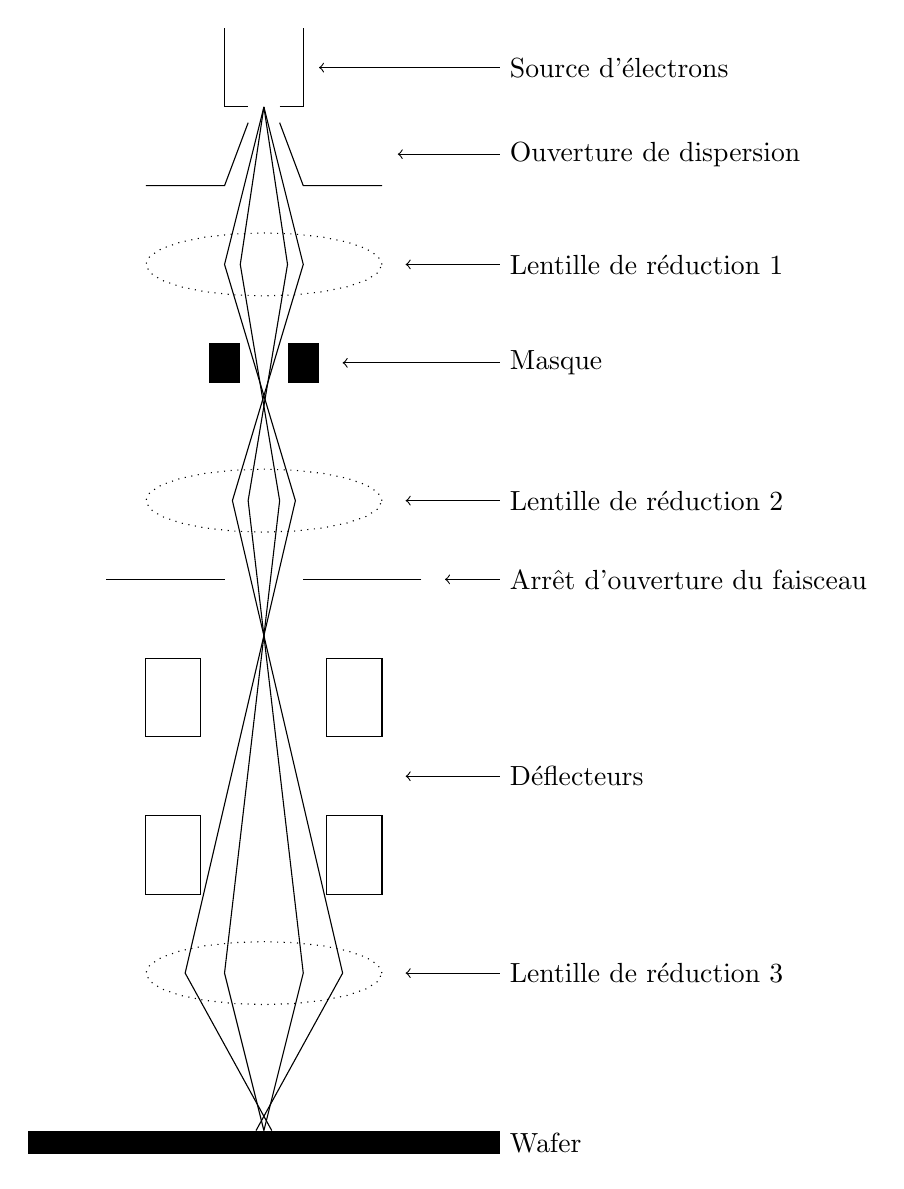
\begin{tikzpicture}
                    \draw (4.5,20)--(4.5,19)--(4.8,19);
                    \draw (5.2,19)--(5.5,19)--(5.5,20);
                    \draw [<-] (5.7,19.5)--(8,19.5);
                    \draw (8,19.5)node[right]{Source d'électrons};
                    
                    \draw (3.5,18)--(4.5,18)--(4.8,18.8);
                    \draw (6.5,18)--(5.5,18)--(5.2,18.8);
                    \draw [<-] (6.7,18.4)--(8,18.4);
                    \draw (8,18.4)node[right]{Ouverture de dispersion};
                    
                    \draw [dotted] [domain=0:360] plot({1.5*cos(\x)+5},{0.4*sin(\x)+17)});
                    \draw [<-] (6.8,17)--(8,17);
                    \draw (8,17)node[right]{Lentille de réduction 1};
                    
                    \fill (4.7,16)--(4.7,15.5)--(4.3,15.5)--(4.3,16)--cycle;
                    \fill (5.3,16)--(5.3,15.5)--(5.7,15.5)--(5.7,16)--cycle;
                    \draw [<-] (6,15.75)--(8,15.75);
                    \draw (8,15.75)node[right]{Masque};
                    
                    \draw [dotted] [domain=0:360] plot({1.5*cos(\x)+5},{0.4*sin(\x)+14)});
                    \draw [<-] (6.8,14)--(8,14);
                    \draw (8,14)node[right]{Lentille de réduction 2};
                    
                    \draw (3,13)--(4.5,13);
                    \draw (7,13)--(5.5,13);
                    \draw [<-] (7.3,13)--(8,13);
                    \draw (8,13) node[right]{Arrêt d'ouverture du faisceau};
                    
                    \draw (3.5,12)--(4.2,12)--(4.2,11)--(3.5,11)--cycle;
                    \draw (6.5,12)--(5.8,12)--(5.8,11)--(6.5,11)--cycle;
                    \draw (3.5,10)--(4.2,10)--(4.2,9)--(3.5,9)--cycle;
                    \draw (6.5,10)--(5.8,10)--(5.8,9)--(6.5,9)--cycle;
                    \draw [<-](6.8,10.5)--(8,10.5);
                    \draw (8,10.5)node[right]{Déflecteurs};
                                                            
                    \draw [dotted] [domain=0:360] plot({1.5*cos(\x)+5},{0.4*sin(\x)+8)});
                    \draw [<-] (6.8,8)--(8,8);
                    \draw (8,8)node[right]{Lentille de réduction 3};
                    
                    \fill (2,6)--(8,6)--(8,5.7)--(2,5.7)--cycle;
                    \draw (8,5.85) node[right]{Wafer};
                    
                    \draw (5,19)--(4.5,17)--(5.4,14)--(4,8)--(5.1,6);
                    \draw (5,19)--(5.5,17)--(4.6,14)--(6,8)--(4.9,6);
                    \draw (5,19)--(4.7,17)--(5.2,14)--(4.5,8)--(5,6);
                    \draw (5,19)--(5.3,17)--(4.8,14)--(5.5,8)--(5,6);
                    \end{tikzpicture}
                    \caption{Schéma fonctionnel simplifié de l'EBL}
                    \label{EBLschema}
            \end{figure}
            
            \begin{figure}
                \centering
                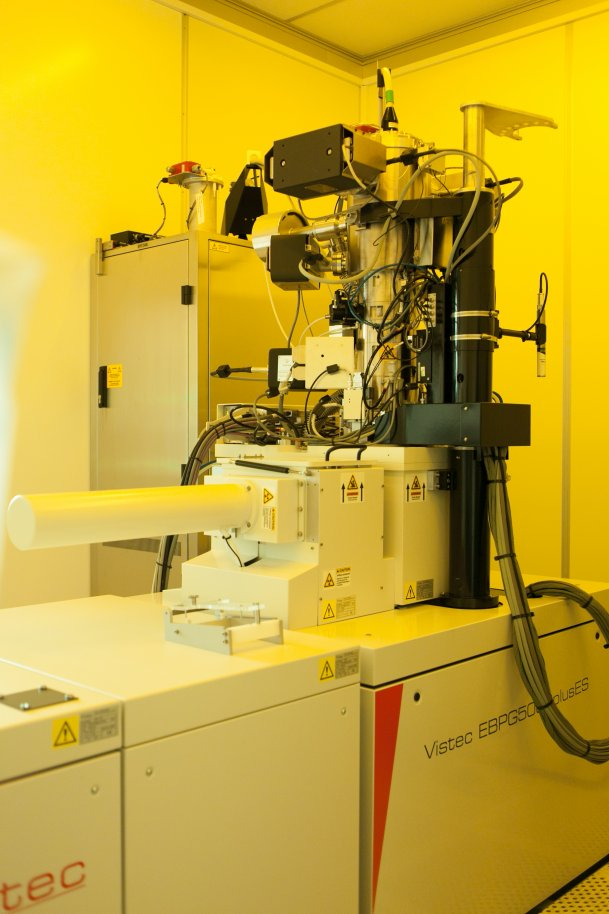
\includegraphics[width=250pt]{EBL.jpg}
                \caption{Photographie de l'Electron Beam Lithographier de la Salle Blanche Nanofab}
            \end{figure}
            
        \subsection{Tracé du pattern}
            Le faisceau peut être controlé informatiquement, via logiciel, on créé notre pattern et on peut ainsi dessiner directement sur le wafer des pattern nanoscopiques. Le faisceu d'électrons altère la résine dans les zones souhaitées, comme le montre la vue en coupe en Fig. \ref{waferEBL}
            
            \begin{figure}
                \centering
                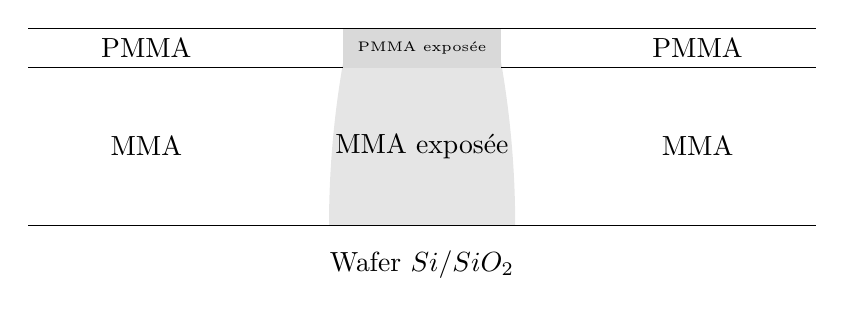
\begin{tikzpicture}
                \draw (5,-0.5) node{Wafer $Si/SiO_2$};
                \fill [color=gray!20] (3.82,0) arc(180:170:12)--++(2,0) arc (10:0:12)--cycle;
                \draw (0,2)--(4,2);
                \draw (6,2)--(10,2);
                \draw (1.5,1) node{MMA};
                \draw (8.5,1) node{MMA};
                \draw (1.5,2.25) node{PMMA};
                \draw (8.5,2.25) node{PMMA};
                \fill [color=gray!30] (4,2)--(4,2.5)--(6,2.5)--(6,2)--cycle;
                \draw (0,2.5)--(10,2.5);
                \draw (5,2.25)node{{\tiny PMMA exposée}};
                 \draw (0,0)--(10,0);
                \draw (5,1)node{MMA exposée};
                \end{tikzpicture}
                \caption{Vue en coupe du wafer après passage dans l'EBL}
                \label{waferEBL}
            \end{figure}
        
        \subsection{Développement}
            Le développement consiste au retrait de la résine exposée à l'EBL. Réalisé par une succession de réactions chimiques, on perce tout d'abord le PMMA avant d'attaquer le MMA pour réaliser ce qu'on appelle des undercut, le MMA étant plus sensible, il est plus atteint et on forme un cône sous le PMMA où la structure prendra place. Les deux résines réagissent au MIBK, qui peut les dissoudre. En effet, en attendant suffisamment longtemps, la résine disparait complètement si elle reste dans la solution de MIBK. En revanche, la partie exposée au faisceau d'électrons est bien plus sensible. Les liaisons étant déjà fragilisées, il suffit de très peu de temps pour retirer la partie souhaitée. À ce moment, la résine de la zone exposée a disparu. Cependant, ce n'est pas suffisant, on souhaite créer une surface accessible /!\ A CHANGER plus grande pour déposer selon un angle précis. C'est le rôle du méthyl glycol. Ce dernier va attaquer selectivement le MMA, et créer ce qu'on appelle des undercuts : une partie du MMA sous le PMMA encore existant est rongée, ce qui crée un dôme sous la PMMA (Fig. \ref{Aprèsdvpt}).
            \begin{figure}
            \centering
            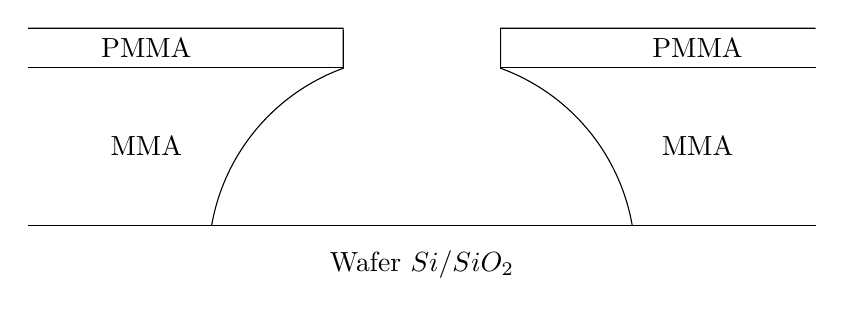
\begin{tikzpicture}
                \draw (0,0)--(10,0);
                \draw (5,-0.5) node{Wafer $Si/SiO_2$};
                \draw (2.33,0) arc(170:110:2.6)--(4,2.5)--(0,2.5);
                \draw (7.67,0) arc(10:70:2.6)--(6,2.5)--(10,2.5);
                \draw (0,2)--(4,2);
                \draw (6,2)--(10,2);
                \draw (1.5,1) node{MMA};
                \draw (8.5,1) node{MMA};
                \draw (1.5,2.25) node{PMMA};
                \draw (8.5,2.25) node{PMMA};
            
            \end{tikzpicture} 
            \caption{Vue en coupe après le développement}
            \label{Aprèsdvpt}
            \end{figure}
            
    \section{Evaporateur}
        \subsection{Fonctionnement de l'évaporateur}
            L'évaporateur permet de déposer un fine couche uniforme de métal à l'intérieur des undercuts fraichement développées. Un filament est soumis à un fort courant et une forte tension, il émet des photons qui vont faire fondre le metal puis en arracher des atomes. Ces atomes se dispersent dans la chambre, et comme le libre parcours moyen est grand, finissent par se déposer uniformément partout. Il y a des capteurs d'épaisseur permettant de fixer l'épaisseur que l'on souhaite atteindre. L'évaporateur possède une valve pour l'oxygène, cela permet d'oxyder les métaux si on souhaite réaliser des jonctions avec isolant par exemple. Il y a également une valve pour injecter de l'argon et réaliser ainsi un plasma au sein de la chambre. Ce plasma possède plusieurs utilités : simplifier le lift-off en fragilisant légèrement la résine. Nous l'avons principalement utilisé pour réaliser du plasma etching : le retrait de matière par plasma. Cela fait partie des tests réalisés en vue d'intégrer les nanofils à une structure permettant leur caractérisation.
            
            \begin{figure}
                \centering
                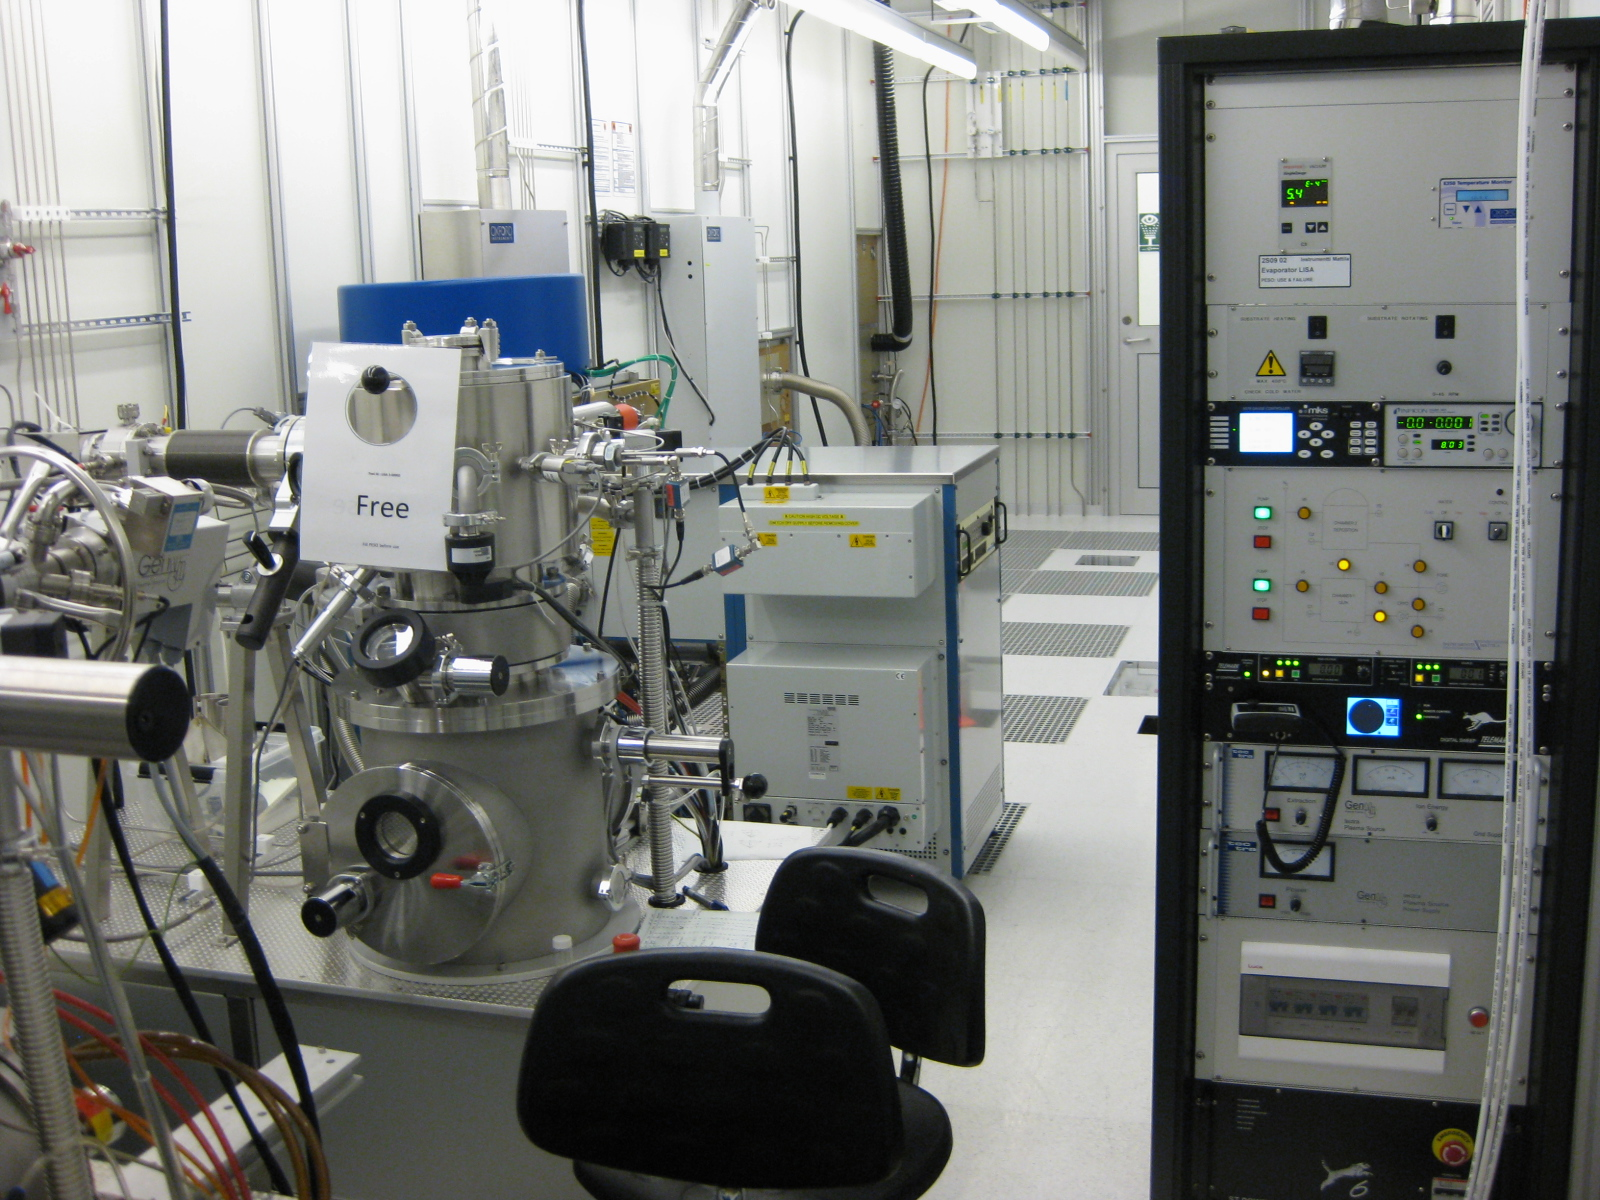
\includegraphics[width=350pt]{LISA.JPG}
                \caption{Photographie de l'évaporateur LISA utilisé pour réaliser les structures}
            \end{figure}
        
    \section{Lift-off et SEM}
        \subsection{Le Lift-off : retrait de la résine}
            Le métal s'est déposé partout suite à l'évaporation, cependant, dans la plupart des endroits, il est sur la résine, il nous suffit ainsi de retirer celle-ci pour avoir nos structures. C'est le rôle de l'acétone qui va dissoudre totalement la résine et ainsi décoller du wafer le métal déposé par évaporation en dehors des zones souhaitées, cette étape s'appelle lift-off.
            
        \subsection{Fonctionnement du SEM}
            Le fonctionnement du SEM est très similaire à celui de l'EBL : on envoie un faisceau d'électrons sur la matière, sauf que cette fois-ci, on ne cherche pas à fragiliser la matière mais à observer la dispersion des électrons dans les échantillons. Chaque matériau ne disperse pas les électrons de la même manière (en particulier, isolant et métal), on peut ainsi observer un contraste entre de la matière isolante et du métal. De plus, le SEM possède un mode "électrons secondaires" qui permet de repérer les électrons créés au sein du matériau. Ces électrons sont différents selon l'élement chimique qui compose le matériau. Ce mode permet de distinguer le cuivre de l'aluminium par exemple. Cependant, ces électrons créés étant peu nombreux, ce mode est plus soumis au bruit et beaucoup plus sombre.
            
            \begin{figure}
                \centering
                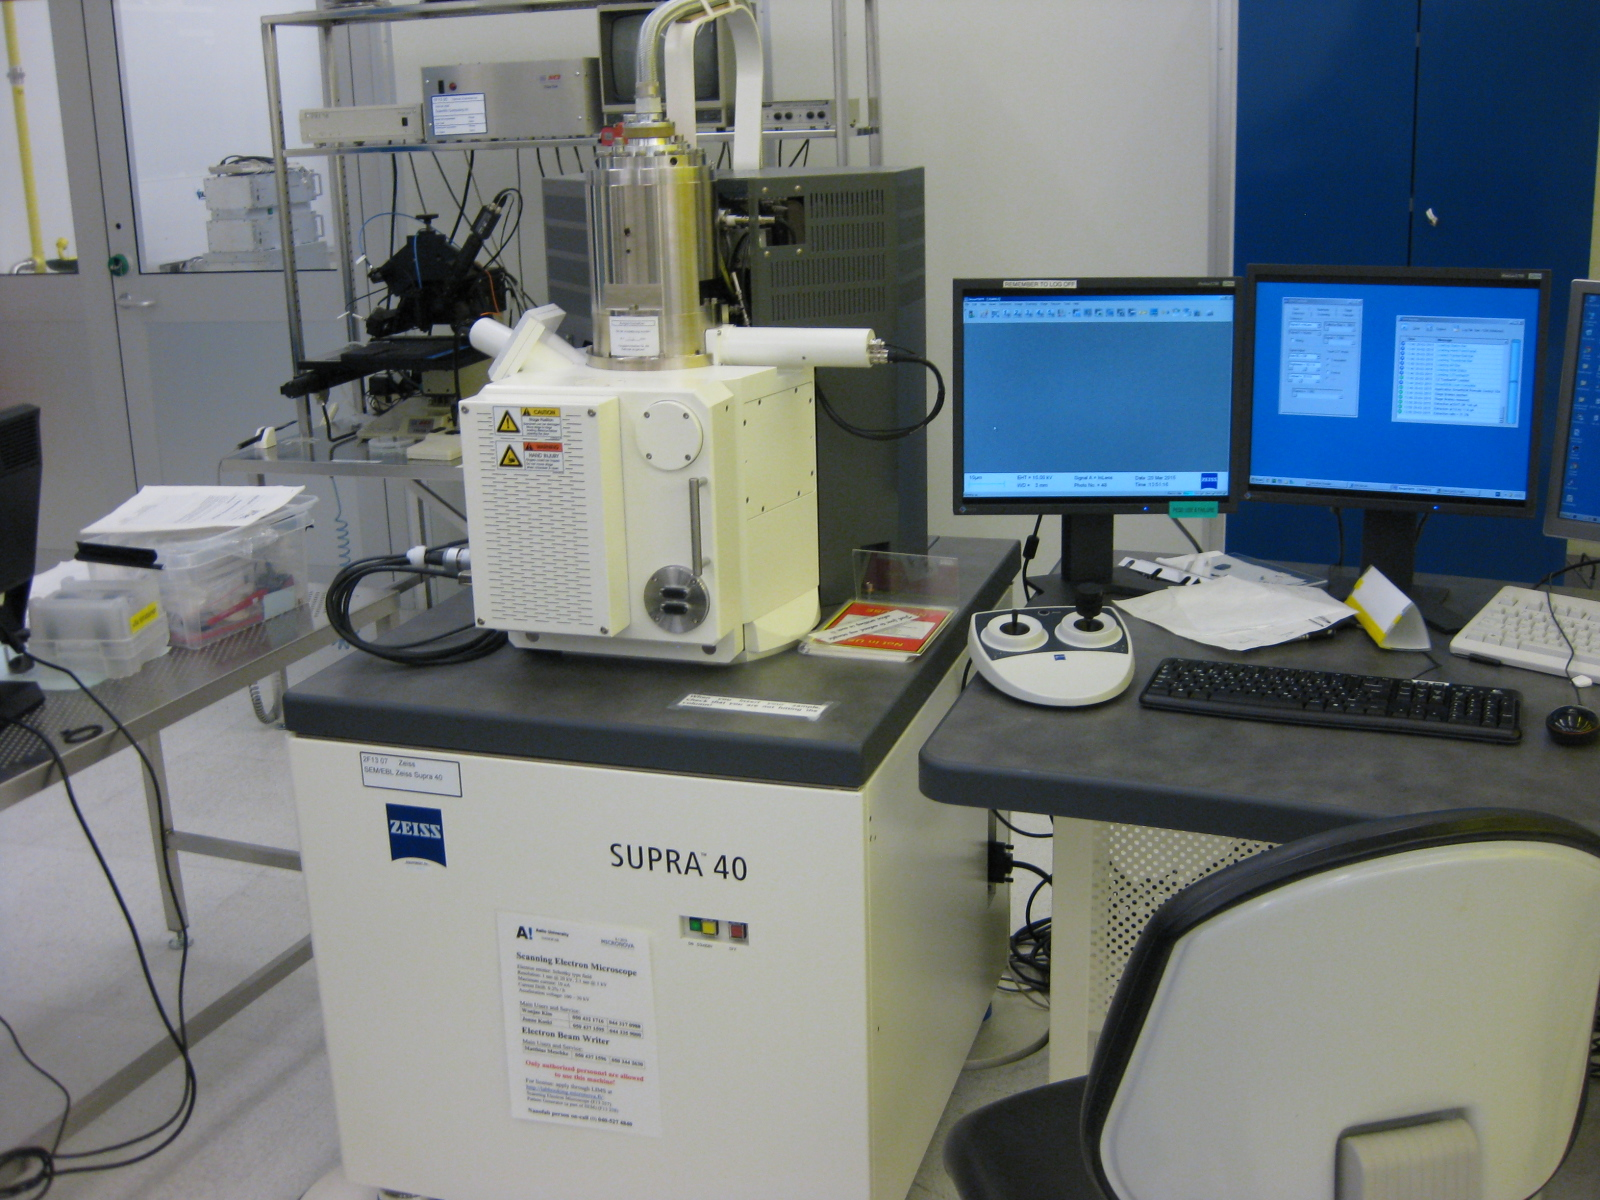
\includegraphics[width=350pt]{SEM.JPG}
                \caption{Photographie du Scanning Electron Microscope utilisé pour observer les structures réalisées}
            \end{figure}
        \subsection{Observation d'échantillons}
            Avant de pouvoir observer distinctement les échantillons, un certains nombre de réglages sont à faire, ressemblant beaucoup à des réglages d'optique : focale, stigmatisme, ouverture... Lorsque l'on réalise les réglages, on choisira un endroit exempt d'échantillons sur le wafer car le SEM envoie des électrons dans la matière et donc la charge. En choisissant un autre endroit (contenant tout de même de la matière autre que le wafer), on éviter de charger nos echantillons. On commence par régler la focale et on tente de faire le point sur l'échantillon. Puis, on régle le stigmatisme en fonction de cette focale. On cherche à obtenir l'image la plus nette possible avant de passer à l'observation des échantillons et la prise d'images comme en Fig.\ref{SEMexemple}.
            
            \begin{figure}
                \centering
                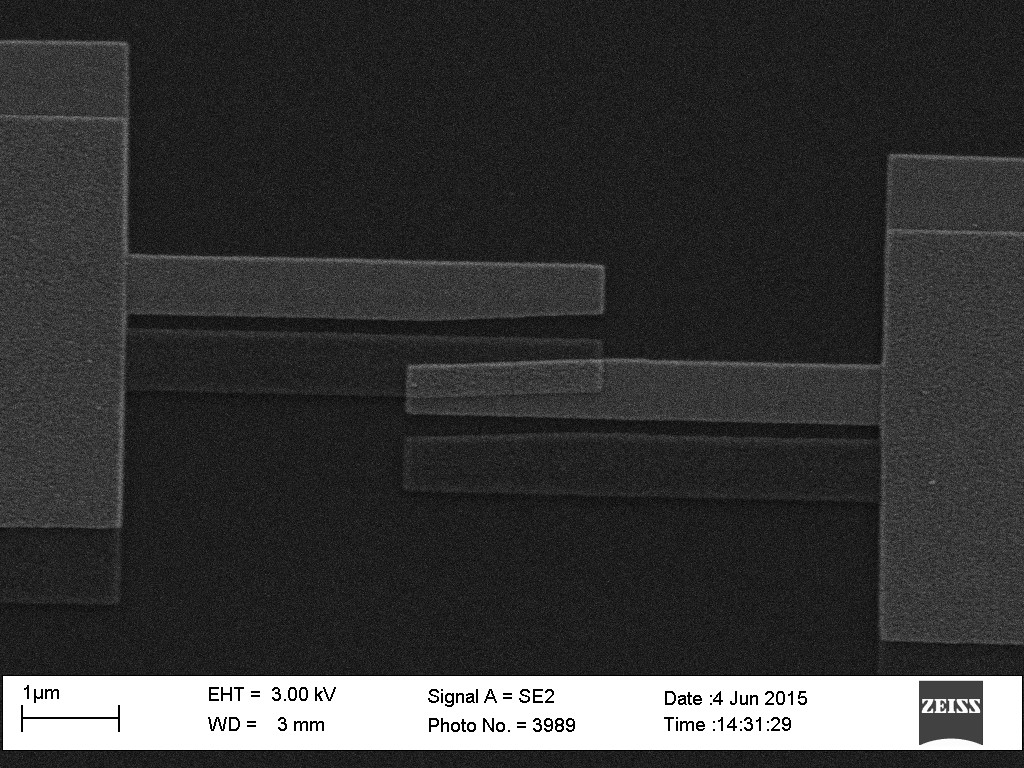
\includegraphics[width=300pt]{SEMexemple.jpg}
                \caption{Exemple d'une structure observée au SEM}
                \label{SEMexemple}
            \end{figure}
